\documentclass[aspectratio=169]{beamer}

\title{PyPI Trusted Publishing}
\author{David Fischer}
\date{November 19, 2026}

%% Beamer Themes
\usetheme{Berlin}
\usecolortheme{dove}
\usefonttheme{serif}

%% Packages
% Pygments must be accessible to use minted and --shell-escape
%  must be used with pdflatex
\usepackage{minted}
\usepackage{hyperref}
\usepackage[T1]{fontenc}
\usepackage{lmodern}
\usepackage[utf8]{inputenc}
\usepackage[font=scriptsize,labelformat=empty]{caption}


\beamertemplatenavigationsymbolsempty
\setbeamertemplate{footline}{
  \hspace*{.2cm}
  \scriptsize{
    \insertshorttitle
    \hspace*{50pt}
    \hfill
    \insertframenumber/\inserttotalframenumber
    \hspace*{.2cm}
  }
  \vspace{9pt}
}

\newsavebox{\blockquotebox}
\newcommand{\blockquoteauthor}{}
\newenvironment{blockquote}[1][]{%
  \renewcommand{\blockquoteauthor}{#1}%
  \begin{lrbox}{\blockquotebox}%
  \begin{minipage}{0.84\textwidth}%
    \vspace*{0.8em}%
    \raggedright\itshape\linespread{1.25}\selectfont
}{%
    \ifx\blockquoteauthor\empty\else
      \par\vspace{0.9em}%
      {\raggedleft\normalfont\small\color{black!65}--- \blockquoteauthor\par}%
    \fi
    \vspace{0.8em}%
  \end{minipage}%
  \end{lrbox}%
  \begin{center}%
    \setlength{\fboxsep}{0pt}%
    \colorbox{black!4}{%
      {\color{black!45}\vrule width 3pt}%
      \hspace{1.4em}%
      \usebox{\blockquotebox}%
      \hspace{1.4em}%
    }%
  \end{center}%
}


\begin{document}

\maketitle


\begin{frame}
\frametitle{What is PyPI Trusted Publishing?}
  \begin{blockquote}[\href{https://blog.pypi.org/posts/2023-04-20-introducing-trusted-publishers/}{the PyPI blog post introducing Trusted Publishing}]
    ``Trusted Publishing'' is [PyPI's] term for using the OpenID Connect (OIDC) standard to exchange short-lived identity tokens between a trusted third-party service and PyPI. This method can be used in automated environments and eliminates the need to use manually generated API tokens to authenticate with PyPI when publishing.
  \end{blockquote}
\end{frame}


\begin{frame}
\frametitle{Why use Trusted Publishing?}

\begin{itemize}
  \item {\scriptsize You publish packages to PyPI (or another package index)}
  \item {\scriptsize You want consistent releases from your CI/CD pipeline}
  \item {\scriptsize You don't want long lived API tokens stored in your CI/CD environment}
  \item {\scriptsize You want a cryptographically verified link between source code and the published package}
  \item {\scriptsize You want digital attestations (PEP 740) - cryptographic proof how a package was built and published}
\end{itemize}

\end{frame}


\begin{frame}[fragile]
\frametitle{Step 1: Configure your CI/CD environment}

{\tiny
\begin{minted}{yaml}
## .github/workflows/release.yml

name: Release

# This workflow is triggered when a "Release" is created from git tag
on:
  release:
    types: [published]

jobs:
  pypi-publish:
    name: Upload release to PyPI
    runs-on: ubuntu-latest
    environment: pypi  # Layer security on top by requiring approvals for this env
    permissions:
      id-token: write  # Required for PyPI Trusted Publishing (OIDC)
    steps:
      - uses: actions/checkout@v4  # Pinning recommended - not shown in this example
      - name: Install uv
        uses: astral-sh/setup-uv@v5
      - name: Set up Python
        run: uv python install
      - name: Build package  # Recommend building in a separate "job"
        run: uv build
      # Use pypa/gh-action-pypi-publish for PEP 740 digital attestations
      - name: Publish to PyPI
        run: uv publish --trusted-publishing always  # No more ${{ secrets.PYPI_TOKEN }}
\end{minted}
}

\end{frame}


\begin{frame}
  \frametitle{Step 2: Configure PyPI Trusted Publishing}
  \begin{figure}[p]
    \centering
    \fbox{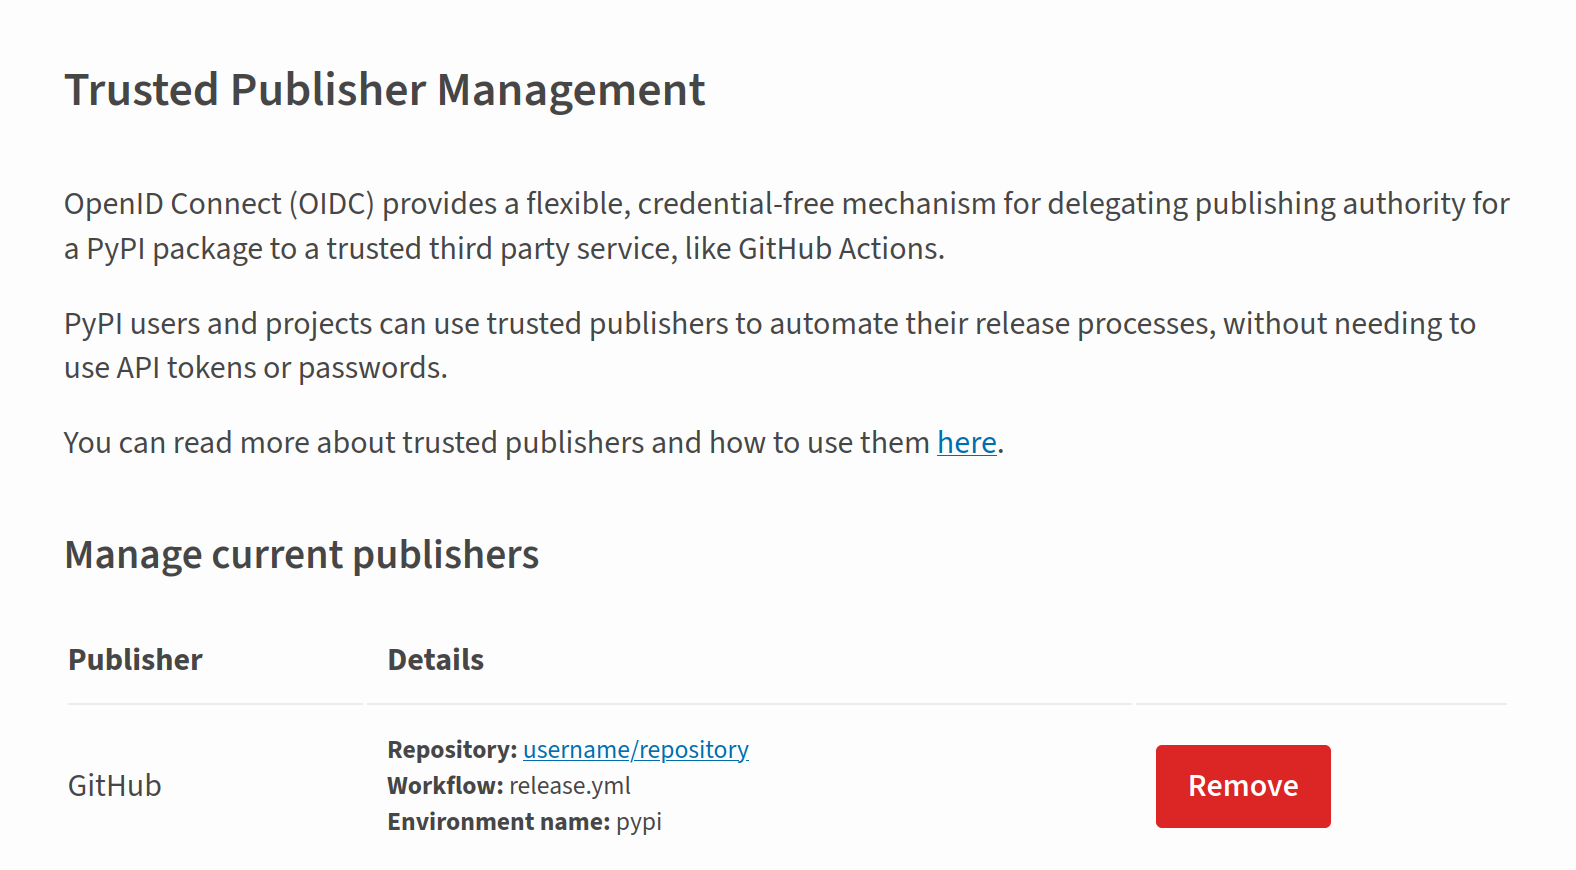
\includegraphics[height=0.5\paperheight]{images/pypi-configuration.png}}
    % GitLab, Google OIDC and ActiveState are also supported
    \caption{\tiny{Configuring trusted publishing on PyPI.org for a GitHub Actions workflow}}
  \end{figure}
\end{frame}



\begin{frame}
\frametitle{Resources}
  \begin{itemize}
    \item {\small \href{https://blog.pypi.org/posts/2023-04-20-introducing-trusted-publishers/}{PyPI Trusted Publishers blog post: https://blog.pypi.org/posts/2023-04-20-introducing-trusted-publishers/}}
    \item {\small \href{https://docs.pypi.org/trusted-publishers/}{PyPI Trusted Publishers docs: https://docs.pypi.org/trusted-publishers/}}
    \item {\small \href{https://peps.python.org/pep-0740/}{PEP 740: Digital Attestations: https://peps.python.org/pep-0740/}}
  \end{itemize}
\end{frame}


\begin{frame}
\frametitle{}
  {\huge Questions?}
\end{frame}


\end{document}
